% Gabarit pandoc des corrigés publiés (brut et guidé). Contenu sans marque ni nom de site.
% Compilation : lualatex (latexmk -lualatex).
% Le Markdown reste la source unique : ne pas éditer ce fichier .tex à la main.
\documentclass[11pt,a4paper]{article}

% --- Moteur, polices (Latin Modern) et langue ---------------------------------
\usepackage{iftex}
\ifLuaTeX\else\errmessage{Ce document se compile avec lualatex}\fi
\usepackage{amsmath,amssymb,mathtools}
\usepackage{fontspec}
% mathrm=sym : \mathrm prend ses glyphes dans la police mathématique (ℓ, μ, Ω), comme KaTeX.
\usepackage[math-style=TeX,bold-style=TeX,mathrm=sym]{unicode-math}
% Repli pour les glyphes absents de Latin Modern (indices et exposants Unicode,
% flèches, filets des schémas en texte, symboles) : DejaVu, puis Latin Modern Math
% (ℓ, lettres mathématiques Unicode des légendes).
\directlua{
  luaotfload.add_fallback("repliTexte", {"DejaVuSerif:mode=harf;", "DejaVuSans:mode=harf;", "file:latinmodern-math.otf:mode=harf;"})
  luaotfload.add_fallback("repliMono", {"DejaVuSansMono:mode=harf;", "DejaVuSans:mode=harf;", "file:latinmodern-math.otf:mode=harf;"})
}
\setmainfont{Latin Modern Roman}[RawFeature={fallback=repliTexte}]
\setsansfont{Latin Modern Sans}[RawFeature={fallback=repliTexte}]
\setmonofont{Latin Modern Mono}[RawFeature={fallback=repliMono}]
\setmathfont{Latin Modern Math}
\usepackage[french]{babel}
\frenchsetup{SmallCapsFigTabCaptions=false}

% --- Mise en page --------------------------------------------------------------
\usepackage[a4paper,margin=2.2cm,headheight=14pt,footskip=1.2cm]{geometry}
\usepackage{microtype}
\setlength{\emergencystretch}{4em}
\tolerance=1500
\setlength{\parindent}{0pt}
\setlength{\parskip}{0.55\baselineskip plus 2pt minus 1pt}
\usepackage{xcolor}
% Gris nommés : babel-french rend « ! » actif dans le document.
\definecolor{gris2}{gray}{0.98}
\definecolor{gris3}{gray}{0.97}
\definecolor{gris5}{gray}{0.95}
\definecolor{gris35}{gray}{0.65}
\definecolor{gris40}{gray}{0.60}
\definecolor{gris45}{gray}{0.55}
\definecolor{gris50}{gray}{0.50}
\definecolor{gris55}{gray}{0.45}
\definecolor{gris60}{gray}{0.40}
\definecolor{gris65}{gray}{0.35}
\definecolor{gris70}{gray}{0.30}
\definecolor{gris80}{gray}{0.20}
\definecolor{gris85}{gray}{0.15}
\usepackage{graphicx}
\usepackage{float}
\usepackage{caption}
\captionsetup{font=small,labelformat=empty,justification=centering}
\usepackage{booktabs,longtable,array,multirow,calc}
\usepackage{siunitx}
\sisetup{locale=FR}
\usepackage[version=4]{mhchem}
\usepackage{listings}
\usepackage{fancyhdr}
\usepackage{lastpage}
\usepackage[most]{tcolorbox}
\usepackage{enumitem}
\setlist{nosep,leftmargin=*,topsep=2pt}
\usepackage[hidelinks,unicode]{hyperref}
\usepackage{bookmark}
\hypersetup{pdftitle={CCINP MP — Mathématiques 1 2026},pdfauthor={Rédigé par IA},pdfcreator={LaTeX},pdfsubject={Corrigé brut}}
\usepackage{xurl}

% --- Pandoc : listes, tableaux, figures ----------------------------------------
\providecommand{\passthrough}[1]{#1}
\providecommand{\tightlist}{\setlength{\itemsep}{0pt}\setlength{\parskip}{0pt}}

\makeatletter
\def\maxwidth{\ifdim\Gin@nat@width>\linewidth\linewidth\else\Gin@nat@width\fi}
\def\maxheight{\ifdim\Gin@nat@height>0.55\textheight 0.55\textheight\else\Gin@nat@height\fi}
\makeatother
\setkeys{Gin}{width=\maxwidth,height=\maxheight,keepaspectratio}
\setcounter{secnumdepth}{-\maxdimen}
\providecommand{\pandocbounded}[1]{#1}

% --- Code (listings) -----------------------------------------------------------
\lstset{
  basicstyle=\ttfamily\small,
  columns=fullflexible,
  keepspaces=true,
  breaklines=true,
  breakatwhitespace=false,
  postbreak=\mbox{\textcolor{gris50}{$\hookrightarrow$}\space},
  frame=single,
  rulecolor=\color{gris35},
  framesep=4pt,
  xleftmargin=5pt,xrightmargin=5pt,
  backgroundcolor=\color{gris3},
  keywordstyle=\bfseries,
  commentstyle=\color{gris65},
  stringstyle=\color{gris80},
  showstringspaces=false,
  tabsize=4,
  extendedchars=true,
  aboveskip=6pt,belowskip=6pt,
}

% --- Macros des corrigés (KaTeX ↔ LaTeX) ---------------------------------------
% Les corrigés sont écrits pour KaTeX : on définit ici ce que KaTeX connaît et
% que LaTeX n'a pas, sans jamais retoucher le Markdown.
\providecommand{\R}{\mathbb{R}}
\providecommand{\N}{\mathbb{N}}
\providecommand{\Z}{\mathbb{Z}}
\providecommand{\Q}{\mathbb{Q}}
\providecommand{\C}{\mathbb{C}}
\providecommand{\dd}{\mathrm{d}}
\providecommand{\llbracket}{\lBrack}
\providecommand{\rrbracket}{\rBrack}
\providecommand{\lBrace}{\lbrace}
\providecommand{\rBrace}{\rbrace}
\providecommand{\Box}{\square}
\providecommand{\Diamond}{\lozenge}
\providecommand{\varnothing}{\emptyset}
\providecommand{\argmax}{\operatorname*{arg\,max}}
\providecommand{\argmin}{\operatorname*{arg\,min}}
\renewcommand{\leq}{\leqslant}
\renewcommand{\geq}{\geqslant}

% Équation hors texte : réduite à la largeur de la ligne si elle déborde.
\newsavebox{\boiteequation}
\newcommand{\equationajustee}[1]{%
  \sbox{\boiteequation}{$\displaystyle #1$}%
  \ifdim\wd\boiteequation>\linewidth
    \[\resizebox{\linewidth}{!}{\usebox{\boiteequation}}\]%
  \else
    \[#1\]%
  \fi}

% --- Encadrés pédagogiques (sobres, lisibles en noir et blanc) -----------------
\tcbset{
  encadre/.style={
    enhanced,breakable,sharp corners,
    colback=white,colframe=gris55,
    boxrule=0.4pt,leftrule=2.2pt,
    left=6pt,right=6pt,top=3pt,bottom=3pt,
    before skip=6pt,after skip=6pt,
    fonttitle=\bfseries\small,coltitle=black,
    attach title to upper,after title={\quad},
    parbox=false,
  }
}
\newtcolorbox{indication}[1]{encadre,colframe=gris45,colback=gris2,title={Indication~#1}}
\newtcolorbox{methode}{encadre,colframe=gris70,title={Méthode}}
\newtcolorbox{piege}{encadre,colframe=gris85,boxrule=0.8pt,leftrule=2.2pt,title={Piège}}
\newtcolorbox{jury}{encadre,colframe=gris60,colback=gris5,title={Jury}}
\newtcolorbox{encadrenote}{encadre,colframe=gris40}

% --- Titres de section ---------------------------------------------------------
\usepackage{titlesec}
\titleformat{\section}{\Large\bfseries}{}{0pt}{}
\titleformat{\subsection}{\large\bfseries}{}{0pt}{}
\titleformat{\subsubsection}{\normalsize\bfseries}{}{0pt}{}
\titlespacing*{\section}{0pt}{14pt plus 4pt minus 2pt}{6pt}
\titlespacing*{\subsection}{0pt}{10pt plus 3pt minus 2pt}{4pt}
\titlespacing*{\subsubsection}{0pt}{8pt plus 2pt minus 2pt}{2pt}

% --- En-tête et pied de page ---------------------------------------------------
\pagestyle{fancy}
\fancyhf{}
\fancyhead[L]{\small\textsc{Corrigé brut} · CCINP MP}
\fancyhead[R]{\small Maths 1 2026}
\fancyfoot[L]{\footnotesize Corrigé rédigé par IA, non officiel}
\fancyfoot[R]{\footnotesize \thepage\,/\,\pageref*{LastPage}}
\renewcommand{\headrulewidth}{0.4pt}
\renewcommand{\footrulewidth}{0pt}
\fancypagestyle{plain}{\fancyhf{}\fancyfoot[R]{\footnotesize \thepage\,/\,\pageref*{LastPage}}\fancyfoot[L]{\footnotesize Corrigé rédigé par IA, non officiel}\renewcommand{\headrulewidth}{0pt}}

\begin{document}
\thispagestyle{plain}
\begin{center}
  {\small\scshape Corrigé brut}\par\smallskip
  {\LARGE\bfseries CCINP MP — Mathématiques 1 2026\par}\medskip
  {\large CCINP · MP · Maths 1 · 2026\par}
\end{center}
\vspace{2pt}\hrule\vspace{8pt}

\emph{Corrigé rédigé par IA, non officiel. Signalez toute erreur.}

Épreuve MP1M1, durée 4 heures, calculatrices interdites. Deux exercices et un problème, 22 questions.

\begin{center}\rule{0.5\linewidth}{0.5pt}\end{center}

\hypertarget{exercice-i}{%
\section{Exercice I}\label{exercice-i}}

Les deux tables sont liées par la clé étrangère \texttt{PAIEMENTS.id\_eleve}, qui référence la clé primaire \texttt{ELEVES.id} : un élève a zéro, un ou plusieurs paiements, un paiement concerne un seul élève.

\begin{figure}[H]
\centering
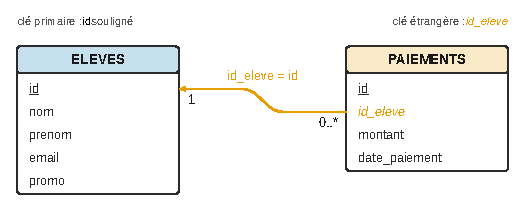
\includegraphics{figures/exo1-schema-tables.pdf}
\caption*{Figure 1 --- Schéma de la base : la clé étrangère id\_eleve de PAIEMENTS
référence la clé primaire id de ELEVES (un élève a 0, 1 ou plusieurs
paiements)}
\end{figure}

\hypertarget{q1}{%
\subsection{Q1}\label{q1}}

Sélection sur \texttt{promo} (opérateur de différence \texttt{\textless{}\textgreater{}}), projection sur \texttt{email}, suppression des doublons par \texttt{DISTINCT} :

\begin{lstlisting}[language=SQL]
SELECT DISTINCT email
FROM ELEVES
WHERE promo <> 2025;
\end{lstlisting}

\hypertarget{q2}{%
\subsection{Q2}\label{q2}}

On joint les deux tables sur \texttt{E.id\ =\allowbreak{}\ P.id\_eleve}, on regroupe par élève (clé primaire \texttt{id}, pour ne pas fusionner deux homonymes) et on somme les montants par \texttt{SUM\ …\ GROUP\ BY}. La jointure externe à gauche conserve les élèves sans paiement :

\begin{lstlisting}[language=SQL]
SELECT E.nom, E.prenom, SUM(P.montant) AS total
FROM ELEVES AS E
LEFT JOIN PAIEMENTS AS P ON E.id = P.id_eleve
GROUP BY E.id, E.nom, E.prenom
ORDER BY E.nom, E.prenom;
\end{lstlisting}

Un élève sans paiement apparaît avec un total \texttt{NULL} (aucun montant à sommer), à lire comme 0. Si l'on se limite aux élèves ayant effectué au moins un paiement, la même requête avec la jointure interne \texttt{JOIN\ PAIEMENTS\ AS\ P\ ON\ E.id\ =\allowbreak{}\ P.id\_eleve} convient.

\hypertarget{q3}{%
\subsection{Q3}\label{q3}}

Deux lignes sont des doublons si elles coïncident sur \texttt{nom}, \texttt{prenom}, \texttt{email}, \texttt{promo} et diffèrent par \texttt{id}. Autojointure :

\begin{lstlisting}[language=SQL]
SELECT DISTINCT E1.id, E1.email
FROM ELEVES AS E1
JOIN ELEVES AS E2
  ON E1.nom = E2.nom AND E1.prenom = E2.prenom
 AND E1.email = E2.email AND E1.promo = E2.promo
WHERE E1.id <> E2.id;
\end{lstlisting}

La condition \texttt{E1.id\ \textless{}\textgreater{}\ E2.id} empêche une ligne de s'apparier avec elle-même ; \texttt{DISTINCT} évite qu'une ligne présente en trois exemplaires ou plus soit affichée plusieurs fois. Variante équivalente par agrégation :

\begin{lstlisting}[language=SQL]
SELECT E.id, E.email
FROM ELEVES AS E
JOIN (SELECT nom, prenom, email, promo
      FROM ELEVES
      GROUP BY nom, prenom, email, promo
      HAVING COUNT(*) >= 2) AS D
  ON E.nom = D.nom AND E.prenom = D.prenom
 AND E.email = D.email AND E.promo = D.promo;
\end{lstlisting}

\hypertarget{q4}{%
\subsection{Q4}\label{q4}}

Un élève sans paiement n'a \textbf{aucune ligne} dans \texttt{PAIEMENTS} ; ce n'est pas un paiement de montant nul, donc un test \texttt{montant\ =\ 0} ne répond pas à la question. Différence ensembliste entre les identifiants d'élèves et les identifiants apparaissant dans \texttt{PAIEMENTS} :

\begin{lstlisting}[language=SQL]
SELECT id FROM ELEVES
EXCEPT
SELECT id_eleve FROM PAIEMENTS;
\end{lstlisting}

Variante par requête imbriquée, équivalente tant que la colonne \texttt{id\_eleve} ne contient pas \texttt{NULL} (sinon \texttt{NOT\ IN} ne renvoie aucune ligne) : \texttt{SELECT\ id\ FROM\ ELEVES\ WHERE\ id\ NOT\ IN\ (\allowbreak{}SELECT\ id\_eleve\ FROM\ PAIEMENTS)\allowbreak{};\allowbreak{}}.

\begin{center}\rule{0.5\linewidth}{0.5pt}\end{center}

\hypertarget{exercice-ii}{%
\section{Exercice II}\label{exercice-ii}}

\hypertarget{q5}{%
\subsection{Q5}\label{q5}}

\(X\) étant à valeurs dans \(\mathbb{N}\), la famille \(\big((X=n)\big)_{n\in\mathbb{N}}\) est un système complet d'événements. La série à termes positifs \(\sum P(X=n)\) converge donc, de somme \(1\).

Soit \(t\in[-1,1]\). Pour tout \(n\in\mathbb{N}\), comme \(|t|\le1\) :

\equationajustee{\begin{aligned}
|P(X=n)t^n|&=P(X=n)|t|^n\\
&\le P(X=n).
\end{aligned}}

Par comparaison de séries à termes positifs, \(\sum P(X=n)t^n\) converge absolument, donc converge.

\textbf{\(G_X\) est bien définie sur \([-1,1]\)} (et même, la majoration étant indépendante de \(t\), la série converge normalement sur ce segment).

\hypertarget{q6}{%
\subsection{Q6}\label{q6}}

Si \(X\hookrightarrow\mathcal{P}(\lambda)\), alors \(P(X=n)={\mathrm{e}}^{-\lambda}\frac{\lambda^n}{n!}\) pour \(n\in\mathbb{N}\). La série exponentielle ayant un rayon de convergence infini, pour tout \(t\in\mathbb{R}\) :

\equationajustee{\begin{aligned}
G_X(t)&=\sum_{n=0}^{+\infty}{\mathrm{e}}^{-\lambda}\frac{(\lambda t)^n}{n!}\\
&={\mathrm{e}}^{-\lambda}{\mathrm{e}}^{\lambda t}.
\end{aligned}}

\equationajustee{\boxed{G_X(t)={\mathrm{e}}^{\lambda(t-1)}}}

\hypertarget{q7}{%
\subsection{Q7}\label{q7}}

Posons \(a_n=P(X=n)\) et \(b_n=P(Y=n)\). Soit \(t\in\,]-1,1[\). D'après Q5, les séries \(\sum a_nt^n\) et \(\sum b_nt^n\) convergent absolument. Par le théorème du produit de Cauchy, leur produit de Cauchy converge absolument et

\equationajustee{G_X(t)G_Y(t)=\sum_{n=0}^{+\infty}c_nt^n,}

où l'on a posé

\equationajustee{c_n=\sum_{k=0}^{n}a_kb_{n-k}.}

Soit \(n\in\mathbb{N}\).

Comme \(X\) et \(Y\) sont à valeurs dans \(\mathbb{N}\), l'événement \((X+Y=n)\) est la réunion disjointe finie des événements \((X=k)\cap(Y=n-k)\), pour \(0\le k\le n\).

Par additivité, puis par \textbf{indépendance de \(X\) et \(Y\)} :

\equationajustee{\begin{aligned}
P(X+Y=n)&=\sum_{k=0}^{n}P\big((X=k)\cap(Y=n-k)\big)\\
&=\sum_{k=0}^{n}P(X=k)P(Y=n-k)\\
&=c_n.
\end{aligned}}

\(X+Y\) étant à valeurs dans \(\mathbb{N}\), on a \(\sum_{n\ge0} c_nt^n=G_{X+Y}(t)\). Donc

\equationajustee{\boxed{\forall t\in\,]-1,1[,\quad G_{X+Y}(t)=G_X(t)\,G_Y(t).}}

\hypertarget{q8}{%
\subsection{Q8}\label{q8}}

\(Z=X+Y\) est à valeurs dans \(\mathbb{N}\). D'après Q7 (qui utilise l'indépendance) et Q6, pour \(t\in\,]-1,1[\) :

\equationajustee{\begin{aligned}
G_Z(t)&={\mathrm{e}}^{\lambda(t-1)}{\mathrm{e}}^{\mu(t-1)}\\
&={\mathrm{e}}^{(\lambda+\mu)(t-1)}\\
&=\sum_{n=0}^{+\infty}{\mathrm{e}}^{-(\lambda+\mu)}\frac{(\lambda+\mu)^n}{n!}t^n.
\end{aligned}}

Les séries entières \(\sum P(Z=n)t^n\) et \(\sum {\mathrm{e}}^{-(\lambda+\mu)}\frac{(\lambda+\mu)^n}{n!}t^n\) ont la même somme sur \(]-1,1[\). Par unicité des coefficients d'un développement en série entière (la fonction génératrice caractérise la loi), pour tout \(n\in\mathbb{N}\) :

\equationajustee{P(Z=n)={\mathrm{e}}^{-(\lambda+\mu)}\frac{(\lambda+\mu)^n}{n!}.}

\equationajustee{\boxed{Z=X+Y\hookrightarrow\mathcal{P}(\lambda+\mu).}}

\begin{center}\rule{0.5\linewidth}{0.5pt}\end{center}

\hypertarget{probluxe8me-partie-i---calcul-dune-intuxe9grale}{%
\section{Problème --- Partie I - Calcul d'une intégrale}\label{probluxe8me-partie-i---calcul-dune-intuxe9grale}}

On note \(\varphi(x,t)=\dfrac{x}{x^2+t^2}\) et \(h(x,t)=\varphi(x,t){\mathrm{e}}^{it}\) pour \(x>0\), \(t\in\mathbb{R}\).

\hypertarget{q9}{%
\subsection{Q9}\label{q9}}

Soit \(x>0\). La fonction \(t\mapsto h(x,t)\) est continue sur \(\mathbb{R}\), car le dénominateur est minoré par \(x^2>0\). De plus

\equationajustee{|h(x,t)|=\frac{x}{x^2+t^2}\underset{|t|\to+\infty}{\sim}\frac{x}{t^2},}

fonction intégrable au voisinage de \(\pm\infty\) (Riemann, exposant \(2>1\)). Par comparaison de fonctions positives, \(t\mapsto h(x,t)\) est intégrable sur \(\mathbb{R}\) : \textbf{\(g\) est bien définie sur \(]0,+\infty[\)}.

\hypertarget{q10}{%
\subsection{Q10}\label{q10}}

Soit \(x>0\). L'application \(u\mapsto xu\) est une bijection de \(\mathbb{R}\) sur \(\mathbb{R}\), de classe \({\mathcal{C}}^1\) et strictement croissante ; l'intégrale converge (Q9).

Le changement de variable \(t=xu\), \(\mathrm{d}t=x\,\mathrm{d}u\), donne

\equationajustee{g(x)=\int_{-\infty}^{+\infty}\frac{x\cdot x}{x^2+x^2u^2}{\mathrm{e}}^{ixu}\,\mathrm{d}u,}

d'où

\equationajustee{\boxed{g(x)=\int_{-\infty}^{+\infty}\frac{{\mathrm{e}}^{ixu}}{1+u^2}\,\mathrm{d}u.}}

Par inégalité triangulaire, et puisque \(|{\mathrm{e}}^{ixu}|=1\) :

\equationajustee{\begin{aligned}
|g(x)|&\le\int_{-\infty}^{+\infty}\frac{\mathrm{d}u}{1+u^2}\\
&=\Big[\arctan u\Big]_{-\infty}^{+\infty}\\
&=\pi.
\end{aligned}}

La borne ne dépend pas de \(x\) : \textbf{\(g\) est bornée sur \(]0,+\infty[\), avec \(|g|\le\pi\).}

\hypertarget{q11}{%
\subsection{Q11}\label{q11}}

Soit \((x_p)\) une suite de réels strictement positifs de limite \(0\). On pose \(f_p(u)=\dfrac{{\mathrm{e}}^{ix_pu}}{1+u^2}\).

\begin{itemize}
\tightlist
\item
  Chaque \(f_p\) est continue sur \(\mathbb{R}\).
\item
  Pour tout \(u\), \(f_p(u)\to\dfrac{1}{1+u^2}\) (continuité de l'exponentielle), limite continue.
\item
  Domination : \(|f_p(u)|=\dfrac{1}{1+u^2}\), indépendante de \(p\), intégrable sur \(\mathbb{R}\).
\end{itemize}

Par le théorème de convergence dominée, \(g(x_p)=\int_{\mathbb{R}}f_p\) tend vers \(\int_{\mathbb{R}}\frac{\mathrm{d}u}{1+u^2}=\pi\). Ceci valant pour toute suite, par caractérisation séquentielle de la limite :

\equationajustee{\boxed{\lim_{x\to0^+}g(x)=\pi.}}

\hypertarget{q12}{%
\subsection{Q12}\label{q12}}

On travaille sur la forme initiale : dériver la forme de Q10 en \(x\) ferait apparaître \(iu\,{\mathrm{e}}^{ixu}/(1+u^2)\), non intégrable. Pour \(t\) fixé, \(x\mapsto h(x,t)\) est de classe \({\mathcal{C}}^2\) sur \(]0,+\infty[\), avec

\equationajustee{\frac{\partial h}{\partial x}(x,t)=\frac{t^2-x^2}{(x^2+t^2)^2}{\mathrm{e}}^{it}}

et

\equationajustee{\frac{\partial^2 h}{\partial x^2}(x,t)=\frac{2x(x^2-3t^2)}{(x^2+t^2)^3}{\mathrm{e}}^{it}.}

\begin{itemize}
\tightlist
\item
  Pour tout \(x>0\), \(t\mapsto h(x,t)\) est continue et intégrable (Q9). La fonction \(t\mapsto\partial_xh(x,t)\) est continue et intégrable car \(\left|\partial_xh(x,\allowbreak t)\right|\le\dfrac{x^2+t^2}{(x^2+t^2)^2}=\dfrac{1}{x^2+t^2}\).
\item
  \(t\mapsto\partial_x^2h(x,t)\) est continue. Domination sur tout segment \([a,b]\subset\,]0,+\infty[\) : pour \(x\in[a,b]\), on a \(|2x(x^2-3t^2)|\le 6x(x^2+t^2)\), donc
\end{itemize}

\equationajustee{\begin{aligned}
\left|\frac{\partial^2 h}{\partial x^2}(x,t)\right|&\le\frac{6x}{(x^2+t^2)^2}\\
&\le\frac{6b}{(a^2+t^2)^2},
\end{aligned}}

fonction de \(t\) seule, continue, intégrable sur \(\mathbb{R}\) (équivalente à \(6b/t^4\) en \(\pm\infty\)).

Une domination sur tout \(]0,+\infty[\) est impossible (en \(t=0\), le majorant \(6/x^3\) explose en \(0^+\)) ; elle n'est pas nécessaire, la régularité étant une propriété locale.

Par le théorème de régularité \({\mathcal{C}}^2\) des intégrales à paramètre (domination sur tout segment), \textbf{\(g\) est de classe \({\mathcal{C}}^2\) sur \(]0,+\infty[\)}, et

\equationajustee{\forall x>0,\quad g''(x)=\int_{-\infty}^{+\infty}\frac{\partial^2\varphi}{\partial x^2}(x,t)\,{\mathrm{e}}^{it}\,\mathrm{d}t.}

\hypertarget{q13}{%
\subsection{Q13}\label{q13}}

Avec \(D=x^2+t^2\) :

\equationajustee{\begin{aligned}
\frac{\partial^2}{\partial x^2}\Big(\frac{x}{D}\Big)&=\frac{\partial}{\partial x}\Big(\frac{t^2-x^2}{D^2}\Big)\\
&=\frac{-2xD-4x(t^2-x^2)}{D^3}\\
&=\frac{2x^3-6xt^2}{D^3},
\end{aligned}}

\equationajustee{\begin{aligned}
\frac{\partial^2}{\partial t^2}\Big(\frac{x}{D}\Big)&=\frac{\partial}{\partial t}\Big(\frac{-2xt}{D^2}\Big)\\
&=\frac{-2xD+8xt^2}{D^3}\\
&=\frac{6xt^2-2x^3}{D^3}.
\end{aligned}}

\equationajustee{\boxed{\frac{\partial^2}{\partial x^2}\Big(\frac{x}{x^2+t^2}\Big)+\frac{\partial^2}{\partial t^2}\Big(\frac{x}{x^2+t^2}\Big)=0.}}

Fixons \(x>0\) et posons \(\psi(t)=\varphi(x,t)\), de classe \({\mathcal{C}}^\infty\) sur \(\mathbb{R}\). D'après Q12 et cette identité :

\equationajustee{g''(x)=-\int_{\mathbb{R}}\psi''(t){\mathrm{e}}^{it}\,\mathrm{d}t.}

Les fonctions \(\psi\), \(\psi'(t)=\frac{-2xt}{D^2}\) et \(\psi''\) sont continues et intégrables sur \(\mathbb{R}\).

Elles sont en effet équivalentes respectivement à \(x/t^2\), \(-2x/t^3\) et \(6x/t^4\) en \(\pm\infty\).

Pour \(A>0\), deux intégrations par parties sur \([-A,A]\) donnent

\equationajustee{\int_{-A}^{A}\psi''(t){\mathrm{e}}^{it}\,\mathrm{d}t=\Big[\psi'(t){\mathrm{e}}^{it}\Big]_{-A}^{A}-i\Big[\psi(t){\mathrm{e}}^{it}\Big]_{-A}^{A}+i^2\int_{-A}^{A}\psi(t){\mathrm{e}}^{it}\,\mathrm{d}t.}

Quand \(A\to+\infty\), \(\psi(\pm A)\to0\) et \(\psi'(\pm A)\to0\), et les intégrales convergent. On obtient \(\int_{\mathbb{R}}\psi''(t){\mathrm{e}}^{it}\,\mathrm{d}t=-g(x)\), donc \(g''(x)=g(x)\) :

\equationajustee{\boxed{g\text{ est solution de }y''-y=0\text{ sur }]0,+\infty[.}}

\hypertarget{q14}{%
\subsection{Q14}\label{q14}}

L'équation linéaire homogène à coefficients constants \(y''-y=0\) a pour équation caractéristique \(r^2-1=0\), de racines \(\pm1\).

Sur l'intervalle \(]0,+\infty[\), il existe donc \((\alpha,\beta)\in{\mathbb{C}}^2\) tel que \(g(x)=\alpha{\mathrm{e}}^{x}+\beta{\mathrm{e}}^{-x}\) pour tout \(x>0\).

\begin{itemize}
\tightlist
\item
  Si \(\alpha\neq0\), \(|g(x)|\ge|\alpha|{\mathrm{e}}^{x}-|\beta|\to+\infty\), ce qui contredit \(|g|\le\pi\) (Q10). Donc \(\alpha=0\).
\item
  \(g(x)=\beta{\mathrm{e}}^{-x}\to\beta\) quand \(x\to0^+\), donc \(\beta=\pi\) (Q11).
\end{itemize}

\begin{figure}[H]
\centering
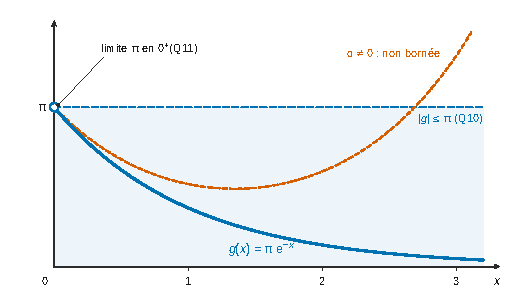
\includegraphics{figures/q14-constantes-g.pdf}
\caption*{Figure 2 --- Q14 : la borne \textbar g\textbar{} ≤ π (Q10) élimine la
composante en e\^{}x, la limite π en 0⁺ (Q11) fixe β = π ; en
pointillés, une solution avec α ≠ 0 qui sort de la bande}
\end{figure}

\equationajustee{\boxed{\forall x>0,\quad g(x)=\pi\,{\mathrm{e}}^{-x}.}}

\hypertarget{partie-ii---formule-sommatoire-de-poisson}{%
\section{Partie II - Formule sommatoire de Poisson}\label{partie-ii---formule-sommatoire-de-poisson}}

\hypertarget{q15}{%
\subsection{Q15}\label{q15}}

Soit \(x\in\mathbb{R}\) fixé. Les termes \(f(x\pm n)\) sont positifs et, quand l'indice \(n\to+\infty\) :

\equationajustee{f(x\pm n)\sim\frac{1}{n^2}.}

Par comparaison à la série de Riemann \(\sum 1/n^2\), les séries \(\sum_{n\ge0}f(x+n)\) et \(\sum_{n\ge1}f(x-n)\) convergent : \textbf{\(F\) est définie sur \(\mathbb{R}\)}.

Périodicité : par décalage d'indice dans des séries convergentes,

\equationajustee{\begin{aligned}
\sum_{n=0}^{+\infty}f(x+1+n)&=\sum_{m=1}^{+\infty}f(x+m)\\
&=\sum_{m=0}^{+\infty}f(x+m)-f(x),
\end{aligned}}

\equationajustee{\begin{aligned}
\sum_{n=1}^{+\infty}f(x+1-n)&=\sum_{m=0}^{+\infty}f(x-m)\\
&=f(x)+\sum_{m=1}^{+\infty}f(x-m).
\end{aligned}}

En additionnant, \(F(x+1)=F(x)\) : \textbf{\(F\) est 1-périodique}.

\hypertarget{q16}{%
\subsection{Q16}\label{q16}}

Posons \(u_n(x)=f(x+n)\) (\(n\ge0\)) et \(v_n(x)=f(x-n)\) (\(n\ge1\)), continues sur \([0,1]\).

Pour \(x\in[0,1]\) et \(n\ge1\) :

\begin{itemize}
\tightlist
\item
  \(x+n\ge n\), donc \(0\le u_n(x)\le\dfrac{1}{1+n^2}\) ;
\item
  \(|x-n|\ge n-1\), donc \(0\le v_n(x)\le\dfrac{1}{1+(n-1)^2}\).
\end{itemize}

Ces majorants sont indépendants de \(x\) et termes généraux de séries convergentes.

Les séries \(\sum u_n\) et \(\sum v_n\) convergent donc normalement, donc uniformément, sur \([0,1]\) (le seul fait que \(\|u_n\|_\infty\to0\) ne suffirait pas). Leurs termes étant continus, \textbf{\(F\) est continue sur \([0,1]\)}.

\begin{figure}[H]
\centering
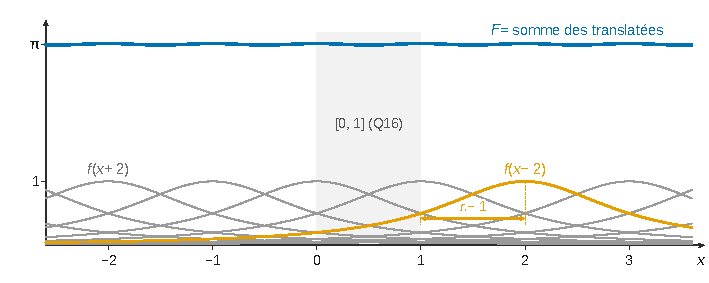
\includegraphics{figures/q15-q16-periodisation.pdf}
\caption*{Figure 3 --- F est la somme des translatées entières de f ; pour 0 ≤ x ≤
1, le pic de f(x − n) est à distance au moins n − 1 (ici n = 2), et F,
quasi constante, vaut π à quelques millièmes près}
\end{figure}

Soit \(k\in\mathbb{Z}\). Pour \(x\in[k,k+1]\), \(F(x)=F(x-k)\) (Q15).

L'application \(x\mapsto F(x-k)\) est continue sur \([k,k+1]\), comme composée de \(x\mapsto x-k\) (à valeurs dans \([0,1]\)) et de \(F_{|[0,1]}\).

Ainsi \(F\) est continue sur chaque \([k,k+1]\), et la continuité en un point non entier en découle.

En un entier \(k\), la continuité sur \([k-1,k]\) et sur \([k,k+1]\) donne les continuités à gauche et à droite. \textbf{\(F\) est continue sur \(\mathbb{R}\).}

\hypertarget{q17}{%
\subsection{Q17}\label{q17}}

\(F\) est continue et 1-périodique, donc \(c_k(F)\) est défini. Soit \(k\in\mathbb{Z}\).

Comme \(|{\mathrm{e}}^{-2i\pi kt}|=1\), les majorations de Q16 montrent que les séries \(\sum f(t+n){\mathrm{e}}^{-2i\pi kt}\) et \(\sum f(t-n){\mathrm{e}}^{-2i\pi kt}\) de fonctions continues convergent uniformément sur le segment \([0,1]\). Par le théorème d'intégration terme à terme sur un segment :

\equationajustee{\begin{aligned}
c_k(F)={}&\sum_{n=0}^{+\infty}\int_0^1f(t+n){\mathrm{e}}^{-2i\pi kt}\,\mathrm{d}t\\
&+\sum_{n=1}^{+\infty}\int_0^1f(t-n){\mathrm{e}}^{-2i\pi kt}\,\mathrm{d}t.
\end{aligned}}

Par la translation \(s=t+n\), et puisque \({\mathrm{e}}^{2i\pi kn}=1\) (\(kn\in\mathbb{Z}\)) :

\equationajustee{\int_0^1f(t+n){\mathrm{e}}^{-2i\pi kt}\,\mathrm{d}t=\int_n^{n+1}f(s){\mathrm{e}}^{-2i\pi ks}\,\mathrm{d}s.}

De même, par \(s=t-n\) et \({\mathrm{e}}^{-2i\pi kn}=1\) :

\equationajustee{\int_0^1f(t-n){\mathrm{e}}^{-2i\pi kt}\,\mathrm{d}t=\int_{-n}^{-n+1}f(s){\mathrm{e}}^{-2i\pi ks}\,\mathrm{d}s.}

La fonction \(s\mapsto f(s){\mathrm{e}}^{-2i\pi ks}\), de module \(f(s)\), est intégrable sur \(\mathbb{R}\).

Par Chasles, les sommes partielles valent \(\int_0^{N+1}\) et \(\int_{-N}^{0}\), qui tendent vers \(\int_0^{+\infty}\) et \(\int_{-\infty}^{0}\). D'où

\equationajustee{\boxed{\forall k\in\mathbb{Z},\quad c_k(F)=\int_{-\infty}^{+\infty}f(t)\,{\mathrm{e}}^{-2i\pi kt}\,\mathrm{d}t.}}

\hypertarget{q18}{%
\subsection{Q18}\label{q18}}

Soient \(k,n\in\mathbb{Z}\) et \(m=n+k\in\mathbb{Z}\). Si \(m=0\), l'intégrande vaut \(1\) et l'intégrale vaut \(1\).

Si \(m\neq0\), comme \({\mathrm{e}}^{-2i\pi m}=1\) (\(m\) entier) :

\equationajustee{\begin{aligned}
\int_0^1{\mathrm{e}}^{-2i\pi mt}\,\mathrm{d}t&=\left[\frac{{\mathrm{e}}^{-2i\pi mt}}{-2i\pi m}\right]_0^1\\
&=\frac{{\mathrm{e}}^{-2i\pi m}-1}{-2i\pi m}\\
&=0.
\end{aligned}}

\equationajustee{\boxed{\int_0^1{\mathrm{e}}^{-2i\pi(n+k)t}\,\mathrm{d}t=\begin{cases}1&\text{si }n+k=0,\\0&\text{sinon.}\end{cases}}}

\hypertarget{partie-iii---applications}{%
\section{Partie III - Applications}\label{partie-iii---applications}}

\hypertarget{q19}{%
\subsection{Q19}\label{q19}}

D'après Q17 avec \(k=0\) :

\equationajustee{c_0(F)=\int_{-\infty}^{+\infty}\frac{\mathrm{d}t}{1+t^2}=\pi.}

Soit \(k\in{\mathbb{N}}^*\). D'après Q17, \(c_k(F)=\displaystyle\int_{-\infty}^{+\infty}\frac{{\mathrm{e}}^{-2i\pi kt}}{1+t^2}\,\mathrm{d}t\). Le changement de variable \(u=-t\) (bijection \({\mathcal{C}}^1\) strictement décroissante de \(\mathbb{R}\) sur \(\mathbb{R}\), intégrale absolument convergente) donne

\equationajustee{c_k(F)=\int_{-\infty}^{+\infty}\frac{{\mathrm{e}}^{2i\pi ku}}{1+u^2}\,\mathrm{d}u.}

C'est \(g(2\pi k)\) d'après Q10 appliquée en \(x=2\pi k>0\). Par Q14 :

\equationajustee{\boxed{\begin{aligned}
c_0(F)&=\pi,\\
\forall k\in{\mathbb{N}}^*,\quad c_k(F)&=\pi\,{\mathrm{e}}^{-2\pi k}.
\end{aligned}}}

Avec le résultat admis \(c_{-k}(F)=c_k(F)\), on a \(c_k(F)=\pi{\mathrm{e}}^{-2\pi|k|}\) pour tout \(k\in\mathbb{Z}\).

\hypertarget{q20}{%
\subsection{Q20}\label{q20}}

Posons \(q={\mathrm{e}}^{-2\pi}\in\,]0,1[\). Pour \(n\in\mathbb{N}\) et \(x\in\mathbb{R}\), d'après Q19 :

\equationajustee{|c_n(F){\mathrm{e}}^{2i\pi nx}|=\pi q^n,}

et de même \(|c_{-n}(F){\mathrm{e}}^{-2i\pi nx}|=\pi q^n\). Ces majorants sont indépendants de \(x\) et termes d'une série géométrique convergente. Les deux séries de fonctions continues convergent normalement, donc uniformément, sur \(\mathbb{R}\) : \textbf{\(G\) est définie et continue sur \(\mathbb{R}\)}.

Chaque terme est 1-périodique car \({\mathrm{e}}^{\pm2i\pi n(x+1)}={\mathrm{e}}^{\pm2i\pi nx}\). Les sommes partielles \(S_N\) de \(G\) vérifient donc \(S_N(x+1)=S_N(x)\) et, par passage à la limite, \textbf{\(G(x+1)=G(x)\)} pour tout \(x\in\mathbb{R}\).

\hypertarget{q21}{%
\subsection{Q21}\label{q21}}

\(F\) (Q15, Q16) et \(G\) (Q20) sont continues sur \(\mathbb{R}\) et 1-périodiques. Par le résultat admis, il suffit de montrer \(c_k(G)=c_k(F)\) pour tout \(k\in\mathbb{Z}\).

Soit \(k\in\mathbb{Z}\). Multipliées par \({\mathrm{e}}^{-2i\pi kt}\) (de module 1), les deux séries définissant \(G\) convergent encore uniformément sur \([0,1]\) ; on intègre terme à terme :

\equationajustee{\begin{aligned}
c_k(G)={}&\sum_{n=0}^{+\infty}c_n(F)\int_0^1{\mathrm{e}}^{-2i\pi(-n+k)t}\,\mathrm{d}t\\
&+\sum_{n=1}^{+\infty}c_{-n}(F)\int_0^1{\mathrm{e}}^{-2i\pi(n+k)t}\,\mathrm{d}t.
\end{aligned}}

D'après Q18, la première intégrale vaut \(1\) si \(n=k\) et \(0\) sinon ; la seconde vaut \(1\) si \(n=-k\) et \(0\) sinon.

\begin{itemize}
\tightlist
\item
  Si \(k\ge0\) : seul le terme \(n=k\) de la première série subsiste ; dans la seconde, \(n=-k\le0\) est exclu. Donc \(c_k(G)=c_k(F)\).
\item
  Si \(k<0\) : dans la première série, \(n=k<0\) est exclu ; dans la seconde, seul \(n=-k\ge1\) subsiste et apporte \(c_{-n}(F)=c_k(F)\). Donc \(c_k(G)=c_k(F)\).
\end{itemize}

Ainsi \(c_k(G)=c_k(F)\) pour tout \(k\in\mathbb{Z}\), et

\equationajustee{\boxed{F=G.}}

\hypertarget{q22}{%
\subsection{Q22}\label{q22}}

Soit \(x\in\mathbb{R}\) et \(z=q\,{\mathrm{e}}^{2i\pi x}\), avec \(|z|=q<1\). D'après Q19 et Q21, en sommant deux séries géométriques convergentes :

\equationajustee{\begin{aligned}
F(x)&=G(x)\\
&=\pi\sum_{n=0}^{+\infty}z^n+\pi\sum_{n=1}^{+\infty}\overline{z}^{\,n}\\
&=\pi\left(\frac{1}{1-z}+\frac{\overline{z}}{1-\overline{z}}\right).
\end{aligned}}

En réduisant au même dénominateur \(|1-z|^2=(1-z)(1-\overline{z})\) :

\equationajustee{\begin{aligned}
\frac{1}{1-z}+\frac{\overline{z}}{1-\overline{z}}&=\frac{1-\overline{z}+\overline{z}-|z|^2}{|1-z|^2}\\
&=\frac{1-q^2}{1-2q\cos(2\pi x)+q^2}.
\end{aligned}}

D'où, avec \(q={\mathrm{e}}^{-2\pi}\), puis en multipliant numérateur et dénominateur par \({\mathrm{e}}^{2\pi}/2\) :

\equationajustee{\boxed{\begin{aligned}
\forall x\in\mathbb{R},\quad F(x)&=\frac{\pi\left(1-{\mathrm{e}}^{-4\pi}\right)}{1-2{\mathrm{e}}^{-2\pi}\cos(2\pi x)+{\mathrm{e}}^{-4\pi}}\\
&=\frac{\pi\,\mathrm{sh}(2\pi)}{\mathrm{ch}(2\pi)-\cos(2\pi x)}.
\end{aligned}}}

Contrôle : en \(x=0\), \(F(0)=\pi\dfrac{1+q}{1-q}=\pi\dfrac{\mathrm{ch}\,\pi}{\mathrm{sh}\,\pi}\), soit \(\displaystyle\sum_{n\in\mathbb{Z}}\frac{1}{1+n^2}=\frac{\pi}{\mathrm{th}\,\pi}\), valeur classique.

\textbf{FIN}

\end{document}
